Habiendo abordado tanto el diseño del sistema como el funcionamiento de los agentes especialistas, este capítulo se centra en los mecanismos de coordinación que permiten la operación del sistema completo.

Para ello se introducirá la lógica del agente principal (MainAgent), el agente planificador y el agente orquestador. Posteriormente se detallarán las variaciones exploradas en dicho marco de coordinación, concluyendo con el análisis de un caso práctico de ejecución.

\section{Agente Principal}
\label{sec:principal}
Este agente establece la lógica de enrutamiento entre el planificador y el orquestador, derivando finalmente el resultado al agente formateador. Todas las versiones principales de este agente pueden visualizarse en la Figura \ref{fig:orchs}.

El proceso se inicia con la ejecución del agente planificador, que genera un plan de alto nivel compuesto por múltiples pasos secuenciales, donde cada paso constituye una cadena de texto que define específicamente qué información buscar. Posteriormente, se activa el agente orquestador con el primer paso del plan generado, cuya función consiste en determinar qué agentes especializados deben ejecutarse para dicha etapa. Los agentes seleccionados son ejecutados de forma asíncrona, generando cada uno un \opus{CitedAIMessage}, estructura que integra tanto el contenido de la respuesta como una lista de citas referentes a los documentos consultados.

Este ciclo se itera hasta que el planificador establece la finalización del plan. A continuación, el agente formateador estructura el contenido en un formato estandarizado, consistente en un mensaje con formato de marcado estructurado (\textit{Markdown}) y un índice de identificadores que referencia solo las citas empleadas de entre todas las generadas en las respuestas de los agentes.

Considerando el desarrollo de múltiples versiones de planificadores y orquestadores, se ha implementado un patrón Builder para facilitar la construcción del sistema a partir de los agentes especificados, permitiendo así las variaciones detalladas en la Sección \ref{sec:vars}. El Listado \ref{lst:builder} muestra la creación, inicialización y ejecución del sistema mínimo con los cinco agentes especialistas.

\begin{lstlisting}[caption={Instanciación y ejecución del sistema mínimo con el patrón Builder},label={lst:builder}]
  builder = FlexibleAgentBuilder()
  agent = await (await (builder
                 .reset()
                 .with_main_agent_type("basic")
                 .with_planner_type("basic")
                 .with_orchestrator_type("basic")
                 .with_specialized_agents([
                      CodeAgent(),
                      CachedConfluenceAgent(),
                      GitlabAgent(),
                      FileSystemAgent(),
                      GoogleDriveAgent(),
                  ])
                 .initialize_agents())).build()

  result = await agent.execute_agent_graph_with_exception_handling({
      "query": "Qué entornos de despliegue existen en el proyecto?",
  })
\end{lstlisting}

\subsection{Respuesta estructurada}
El sistema necesita interpretar las respuestas de los agentes de forma programática en varios escenarios. Para conseguir este objetivo, se implementan respuestas estructuradas que permiten procesar información de manera automatizada dentro de la arquitectura del sistema. Por ejemplo, el agente formateador separa el texto de la respuesta de las citas utilizadas, mientras que el orquestador genera listas de agentes especializados en un formato directamente interpretable por el código.

El Listado \ref{lst:structured_output} muestra la implementación mediante el adaptador \opus{with_structured_output}, que incorpora en el prompt un esquema JSON específico que guía al modelo a generar una salida estructurada. Esta salida, gracias a los modelos Pydantic\footnote{Pydantic: \url{https://docs.pydantic.dev/latest/}}, puede ser automáticamente deserializada a objetos Python para su procesamiento. En los casos donde el modelo no logra producir la estructura correcta, se implementa un mecanismo de recuperación utilizando un \opus{RetryOutputParser} de LangChain, que emplea un segundo modelo para reformular la respuesta según el formato requerido. Si este segundo intento también falla, el proceso se repite hasta obtener una salida válida o llegar al máximo de repeticiones.

\begin{lstlisting}[caption={Validación de la salida estructurada de un LLM},label={lst:structured_output}]
  async def execute_structured_llm_with_validator_handling(prompt: str | Sequence[BaseMessage], output_schema: Type[BaseModel], max_retries: int, llm: BaseChatModel) -> BaseModel:

    structured_model = llm.with_structured_output(output_schema)
    parser = PydanticOutputParser(pydantic_object=output_schema)
    retry_parser = RetryOutputParser.from_llm(parser=parser, llm=default_llm)

    last_exception: Optional[Exception] = None
    raw_response: Optional[str] = None

    for _ in range(max_retries):
        try:
            response = await structured_model.ainvoke(prompt)
            # Validación programática de la salida del modelo 
            raw_response = response if isinstance(response, str) else None
            if not isinstance(response, output_schema):
                response = output_schema.model_validate(response)
            return response

        except Exception as e:
            last_exception = e
            if raw_response is not None:
                try:
                    # Reintento mediante un modelo parseador
                    response = retry_parser.parse(raw_response)
                    if not isinstance(response, output_schema):
                        response = output_schema.model_validate(response)
                    return response
                except Exception as retry_e:
                    last_exception = retry_e
    raise last_exception
\end{lstlisting}

\subsection{Agente Planificador}
\label{sec:agente_planificador}
Este agente establece planes de alto nivel para estructurar el proceso de respuesta mediante un procedimiento lógico secuencial. Adicionalmente, incorpora la capacidad de modificar dinámicamente dichos planes en función del estado de ejecución actual.

El flujo operativo del agente se ilustra en la Figura \ref{fig:planner}. En primera instancia, se verifica que el plan no esté finalizado mediante el condicional \opus{check_current_plan()}. Se considera que un plan ha concluido cuando la ejecución del planificador previo así lo ha determinado o cuando se ha excedido el límite de iteraciones establecido. En caso de detectarse la finalización del plan, se termina inmediatamente la ejecución del planificador.

\begin{figure}[h]
\centering
\adjustbox{center=\textwidth}{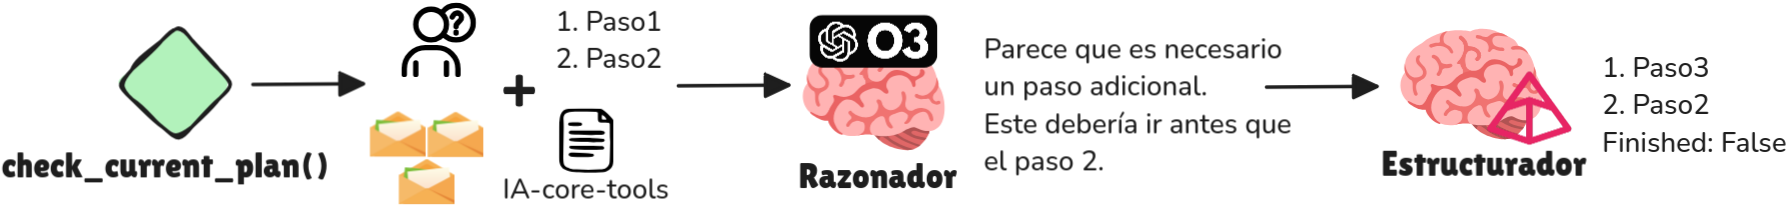
\includegraphics[width=1.25\linewidth]{figures/planner.png}}
\caption{Flujo operativo del agente planificador}
\label{fig:planner}
\end{figure}
Posteriormente, un agente razonador procesa la consulta del usuario junto con una breve descripción del proyecto. En caso de no tratarse de la primera iteración de ejecución, este recibe también los planes anteriores y las respuestas de los agentes especializados, que constituyen el resultado de la ejecución del primer paso de todos los planes precedentes. La función del agente razonador consiste en analizar los siguientes pasos a ejecutar, generando un nuevo plan o modificando el existente.

Cabe destacar que el razonador no estructura directamente su plan, puesto que los agentes razonadores han sido optimizados para generar respuestas sin un formato predeterminado, habiéndose demostrado que imponer restricciones de formato reduce la precisión del razonamiento \cite{tam_let_2024}. Por consiguiente, otro agente, denominado estructurador, transforma el plan textual elaborado por el razonador a un modelo de Pydantic. Este plan consiste en un objeto Python representado como una lista de pasos textuales con un argumento booleano que indica si el plan ha finalizado.

\section{Agente orquestador}
\label{sec:agente_orquestador}
Este agente recibe una tarea específica, ya sea derivada de un paso del plan establecido o formulada como consulta directa por el usuario, y determina qué agentes especializados deben ejecutarse de forma asíncrona.

Para fundamentar su toma de decisiones, su prompt incorpora una descripción detallada de cada agente disponible, incluyendo una síntesis del tipo de información que gestiona cada uno. Este contexto se construye dinámicamente en función de los agentes integrados en el sistema, almacenando dicha caracterización en cada instancia \opus{SpecializedAgent}.

\section{Variaciones de orquestación}
\label{sec:vars}
El sistema base sigue la estructura descrita en la Sección \ref{sec:principal}, donde un orquestador selecciona los agentes a ejecutar para los pasos del plan generados por un planificador. Como se observa en la Figura \ref{fig:orch_1}, este diseño establece una separación completa entre el agente planificador y el agente orquestador. Consecuentemente, el planificador no dispone de información sobre los agentes especialistas disponibles, mientras que el orquestador carece de conocimiento sobre el plan general o la consulta original del usuario, concentrándose exclusivamente en el siguiente paso del plan actual.

\begin{figure}[hbtp]
\centering
\subfloat[Sistema con planificador y orquestador independientes\label{fig:orch_1}]{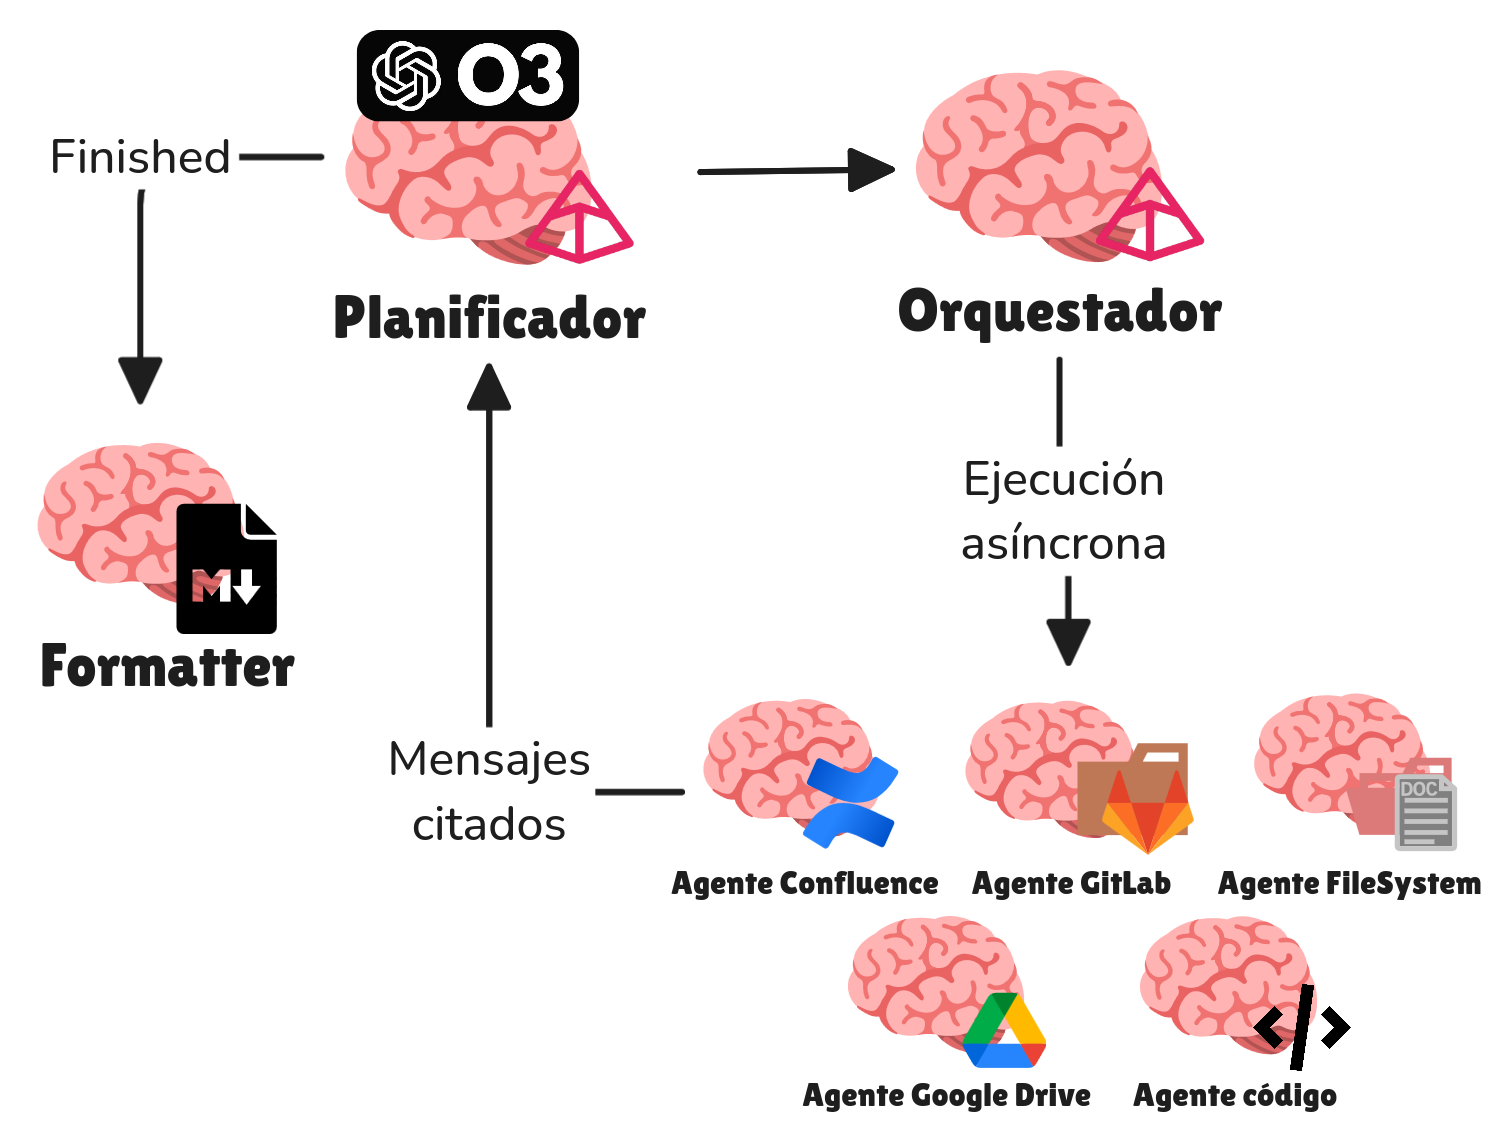
\includegraphics[width=0.6\textwidth]{figures/orch_1.png}}
\hfill
\subfloat[Sistema con planificador y orquestador fusionados\label{fig:orch_2}]{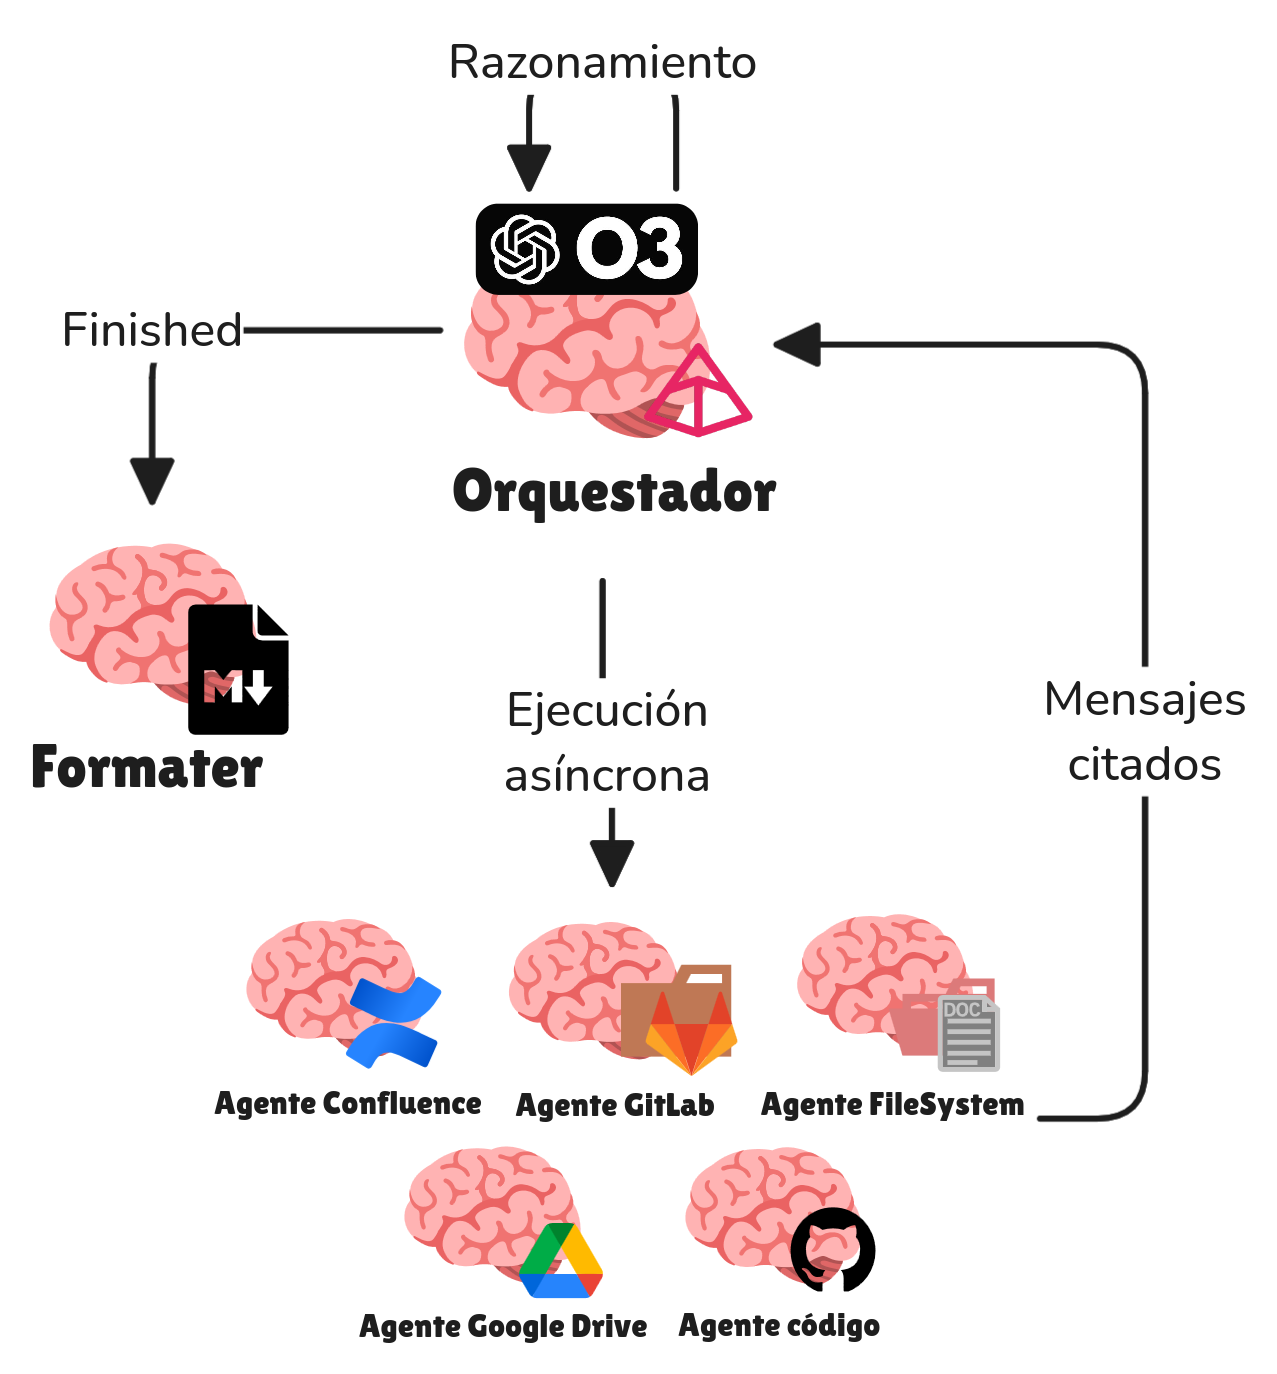
\includegraphics[width=0.5\textwidth]{figures/orch_2.png}}
\hfill
\subfloat[Sistema con orquestador como agente ReAct\label{fig:orch_3}]{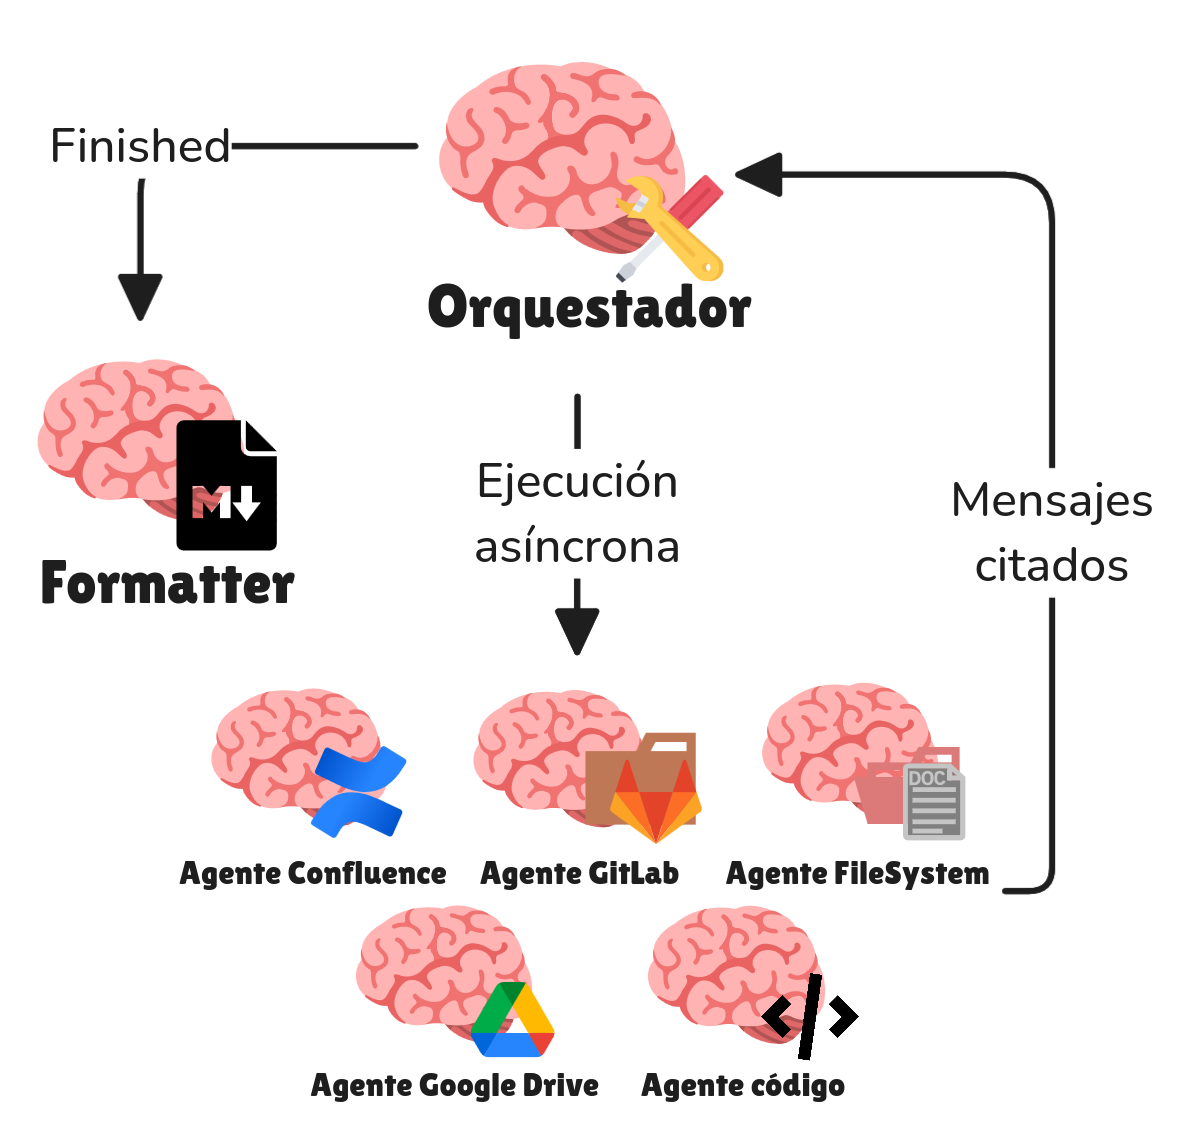
\includegraphics[width=0.5\textwidth]{figures/orch_3.png}}
\caption{Variaciones de orquestación principales experimentadas}
\label{fig:orchs}
\end{figure}

En contraste, la arquitectura ilustrada en la Figura \ref{fig:orch_2} integra el planificador y orquestador en un único agente. Esta fusión permite que disponga de la cuestión del usuario, el plan completo actual y los agentes que puede ejecutar. En esta implementación, tras la fase de razonamiento en el planificador, en lugar de extraer los pasos del plan a ejecutar, se obtienen directamente los agentes a ejecutar con sus respectivas consultas.

Estos dos primeros enfoques presentan ventajas e inconvenientes diferenciados. Mientras que el segundo enfoque resulta más simple y podría presumirse una precisión superior al integrar toda la información contextualizada en un único agente, el primero establece una separación más clara. Esta separación entre planificación y ejecución podría traducirse en decisiones más meditadas, potencialmente mejorando la precisión.

La tercera aproximación, ilustrada en la Figura \ref{fig:orch_3}, explora un diseño de máxima simplicidad. Eliminando completamente la fase de planificación, implementa un orquestador que invoca a los agentes especializados mediante el patrón ReAct, interactuando con ellos encapsulándolos en herramientas. El propio orquestador determina la necesidad de ejecutar agentes adicionales, proporcionando una respuesta directa cuando considera que dispone de información suficiente.

\subsection{Caso práctico}
Para ilustrar el funcionamiento de cada enfoque, esta sección analiza el comportamiento de las diferentes estructuras ante la siguiente consulta del usuario: \texttt{¿Podrías proporcionar ejemplos de código donde se apliquen los principios de la guía de estilos?}

Este ejemplo requiere dos pasos lógicos secuenciales: primero, identificar los principios establecidos en la guía de estilos, lo que implica localizar y extraer el documento completo; posteriormente, analizar qué principios específicos deben buscarse y realizar una exploración en el repositorio para localizar su implementación. La respuesta deberá incluir citas tanto de la guía de estilos como de los archivos que contienen los fragmentos de código incluidos en la respuesta.

\begin{itemize}

\item\textbf{Sistema base: } el planificador genera un plan secuencial de dos pasos: primero localizar la guía de estilos y después identificar su aplicación en el código. Para el primer paso, el orquestador invoca al agente Confluence. El planificador evalúa el resultado obtenido y, si encuentra la guía, autoriza proceder al segundo paso; en caso contrario, modifica el plan para ampliar la búsqueda. Una vez identificada la guía, en el siguiente paso el orquestador consulta al agente de código para localizar la implementación de los principios específicos.

\item\textbf{Sistema unificado:} este implementa un procedimiento similar al sistema básico, pero integrando ambas funciones en cada iteración del orquestador. El agente orquestador establece los dos pasos a ejecutar y, sin delegar en un agente externo, indica directamente la ejecución del agente Confluence para el primer paso. Posteriormente, analiza los resultados obtenidos, modifica el plan de ser necesario y ejecuta el siguiente paso.

\item\textbf{Sistema con orquestador autónomo:} el orquestador recibe la consulta y, sin planificación previa, debe determinar qué agente debe invocarse para obtener la guía de estilos. Tras procesar el resultado, invocará al agente de código para buscar la implementación de los principios identificados.
\end{itemize}

Es relevante destacar las limitaciones del sistema con orquestador autónomo. Aunque presenta mayor simplicidad y rapidez de ejecución, previsiblemente mostrará un rendimiento inferior en escenarios complejos. Al carecer de una fase explícita de reflexión, podría, por ejemplo, invocar al agente de código sin haber localizado correctamente la guía de estilos.
